% Don't modify this section unless you know what you're doing!
\documentclass[letterpaper,12pt]{article}
\usepackage{float}
\usepackage[spanish]{babel}
\selectlanguage{spanish}
\usepackage[utf8]{inputenc}
\usepackage{tabularx} % extra features for tabular environment
\usepackage{amsmath}  % improve math presentation
\usepackage{graphicx, wrapfig, subcaption, setspace, booktabs}
\usepackage{graphicx} % takes care of graphic including machinery

\usepackage[margin=1in,letterpaper]{geometry} % decreases margins
\usepackage{cite} % takes care of citations
\usepackage[final]{hyperref} % adds hyper links inside the generated pdf file
\usepackage{amsmath}
\usepackage{amssymb}
\usepackage{enumerate}
\usepackage{url}
\hypersetup{
	colorlinks=true,       % false: boxed links; true: colored links
	linkcolor=blue,        % color of internal links
	citecolor=blue,        % color of links to bibliography
	filecolor=magenta,     % color of file links
	urlcolor=blue         
}
%++++++++++++++++++++++++++++++++++++++++


\begin{document}

\title{Reporte de la actividad 6}
\author{Daniela Olmos Velderrain\\Grupo 3}
\date{7 de marzo de 2019}

\maketitle

\section{Introducción}
En esta actividad se realizó la comparación de dos modelos distintos utilizados en el cálculo de las horas frío, para estimar el final de la dormancia, es decir, el período durante el cual la semilla de una planta no puede germinar tras caer de su progenitor.
\\
\\
Los datos usados para el análisis provienen de la estación ubicada en un cultivo de Vid, en el Km. 41 de la carretera Hermosillo a Bahía Kino.
\\
\\
El calculo de las horas frío fue realizado por medio de dos modelos diferentes, para después contrastar dichos modelos entre ellos mediante su representación gráfica.  

\section{Desarrollo}
\subsection{Marco teórico}
El requisito de acumulación de frío es un factor en la adaptación de especies frutales caducifolias (como manzanos, perales, durazneros, entre otras) a su ambiente. 
\\
\\
Estas especies deben estar expuestas a bajas temperaturas por un periodo de tiempo durante el letargo invernal, esto para una adecuada ruptura de la dormición e inicio de la nueva estación de crecimiento. 
\\
\\
Existen diferentes modelos para realizar el cálculo de horas frío para cada especie. Nosotros haremos la comparación de dos de estos modelos: el modelo de Utah y el modelo INIFAP-CECH.

\subsubsection{Modelo Utah}
El modelo Utah para el cálculo de horas frío está resumido en la siguiente tabla:


\begin{table}[H]
     &  \\
     & 
\label{tabla:1}
\centering
\caption{Modelo Utah para el cáculo de UF.}
\begin{tabular*}{10 cm}{|l|l@{\extracolsep{\fill}}r|}
\hline
Temperatura ($^\circ C$) & UF correspondiente a 1hr    &\\
\hline
$<$1.4                     &           0.0               &\\
1.5 a 2.4                &           0.5               &\\
2.5 a 9.1                &           1.0               &\\
9.2 a 12.4               &           0.5               &\\
12.5 a 15.9              &           0.0               &\\
16.0 a 18.0              &          -0.5               &\\
$>$18.0                    &          -1.0               &\\
\hline
\end{tabular*}
\end{table}

La suma de UF por día se denota como UF24. Se suman las UF24 a partir del primero de noviembre para cada cultivo.

\subsubsection{Modelo INIFAP-CECH}
El modelo INIFAP-CECH utiliza un algoritmo distinto. Se denomina HF al número de horas frío por día (cuando la temperatura promedio es mayor a $0^\circ C$ y mayor o igual a $10^\circ C$) , y HFE al número de horas frío efectivas por día (se calcula con la diferencia de HF y el número de horas con temperaturas promedio mayores o iguales a $25^\circ C$). Al igual que el modelo Utah, se toma un periodo de tiempo a partir del 1 de noviembre.

\subsection{Metodología} 
Para comenzar a trabajar con el archivo, primero fue necesario descargar librerías para el análisis de datos y visualización:

\begin{verbatim}
import pandas as pd
import numpy as np
import matplotlib.pyplot as plt
\end{verbatim}

El archivo de texto utilizado estaba organizado de manera que los datos se encontraban separados por comas. Esto lo especificamos agregando al el parámetro $delimeter$ al leer el archivo:

\begin{verbatim}
    df0 = pd.read_csv("vid18_180219.dat",delimiter=',')
\end{verbatim}

El documento contaba con 36 parámetros, pero solo nos interesaban los correspondientes a la fecha y la temperatura del aire, así que filtramos estos datos para quedarnos con un data frame más pequeño:

\begin{verbatim}
    df = df0.filter(['TIMESTAMP','AirTC_Avg'],axis=1)
\end{verbatim}

Como las variables requeridas para cada modelo debían calcularse por hora y día, fue necesario convertir la columna de TIMESTAMP a formato de fecha, y posteriormente extraer los datos de año, mes, día y hora en columnas separadas:

\begin{verbatim}
    df['FECHAN'] = pd.to_datetime(df.apply(lambda x: x['FECHA'], 1), dayfirst=True)
    df['AÑO'] = df['FECHA'].dt.year
    df['MES'] = df['FECHA'].dt.month
    df['DIA'] = df['FECHA'].dt.day
    df['HORA'] = df['FECHA'].dt.hour
\end{verbatim}

Se pide que el análisis de datos se realice a partir del primero de noviembre, así que restringimos el data frame a los valores después de esta fecha:

\begin{verbatim}
    df = df[(df['FECHA'] >= "2018-11-1")]
\end{verbatim}

Los datos de temperatura en el archivo fueron tomados cada 10 minutos, sin embargo, los parámetros requeridos son la temperatura promedio cada hora, así como la temperatura máxima y mínima diaria. Por tanto, hicimos uso de las funciones $groupby$ y $transform$, para agrupar los datos y encontrar su promedio y valores máximos y mínimos:

\begin{verbatim}
df["TEMPROM"] = np.round(df.groupby(["AÑO","MES","DIA","HORA"])["AirTC_Avg"]
.transform("mean"),decimals=1)

df["TMAX"] = np.round(df.groupby(["AÑO","MES","DIA"])["AirTC_Avg"].transform
("max"),decimals=1)

df["TMIN"] = np.round(df.groupby(["AÑO","MES","DIA"])["AirTC_Avg"]
.transform
("min"),decimals=1)
\end{verbatim}

Como contábamos con valores repetidos, ya que solo nos interesaban parámetros calculados cada hora, usamos una función para quitar estos datos duplicados, y otra para crear un nuevo índice:

\begin{verbatim}
    df = df.drop_duplicates(subset=['AÑO','MES','DIA','HORA'])
    df=df.reset_index(drop=True)
\end{verbatim}

Ahora, llenamos arreglos mediante condicionales basados en los estándares propuestos para cada modelo.
\\
\\
Para el modelo de Utah se llenó el arrreglo UF que contenía las unidades de frío por hora.
\\
\\
Para el modelo de INIFAP-CECH se llenaron los arreglos HFhr (arreglo con valores de 0 y 1, asignando el valor de 1 para indicar si la temperatura está entre $0^\circ C$ y $10^\circ C$) y  HChr ( al igual que el anterior con valores de 0 y 1, donde los 1 indican temperaturas promedio mayores o iguales a 25°C).
\\
\\
Se agregaron estos tres arreglos como columnas para el data frame, y se volvieron a aplicar las funciones $groupby$ y $transform$ para obtener la suma de estos valores por día, y colocando los valores obtenidos bajo las etiquetas de UF24, HF y HC.

\begin{verbatim}
df["UF24"] = df.groupby(["AÑO","MES","DIA"])["UF"].transform("sum")
df["HF"] = df.groupby(["AÑO","MES","DIA"])["HFhr"].transform("sum")
df["HC"] = df.groupby(["AÑO","MES","DIA"])["HChr"].transform("sum")
\end{verbatim}

Posteriormente se volvieron a desechar los valores repetidos, esta vez por hora. Finalmente, se calculó el parámetro HFE con la diferencia de los valores de HF y HC: 

\begin{verbatim}
df['HFE']=df.HF-df.HC      
\end{verbatim}

Para realizar las gráficas de evolución, se guardaron los valores de HFE y UF24 en arreglos. También se graficaron las sumas acumuladas de estos arreglos, aplicando la función $cumsum$.

\subsection{Resultados}
A continuación se muestra una visualización de la evolución de los parámetros calculados para cada día:


\begin{center}
	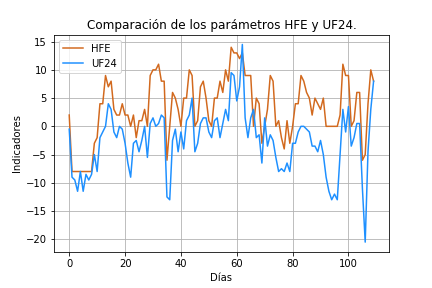
\includegraphics[height=5cm]{HFE_U24.png}\hspace*{\fill}
	\label{graf1}
   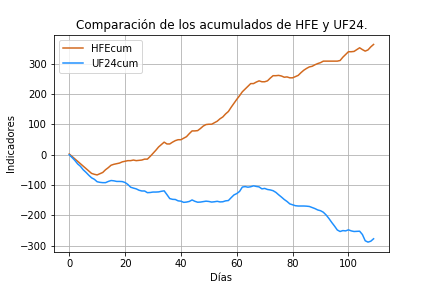
\includegraphics[height=5cm]{HFE_U24_cum.png}
    \label{graf2}
\end{center}


Mientras que las gráficas para los parámetros HFE y UF24 parecen evolucionar de manera semejante, al calcular el acumulado de dichos valores vemos que su comportamiento es completamente diferente. Mientras que el parámetro HFE acumulado tiene un comportamiento creciente, el acumulado de UF24 avanza de manera decreciente. 
\\
\\
Este resultado puede atribuirse a la manera en que son calculados los indicadores. El parámetro UF asigna valores negativos a temperaturas mayores a $16^\circ C$ las cuales son comunes en el clima de Bahía de Kino, de forma que la gráfica para valores acumulados siempre va decreciendo. En cambio, los valores que se restan en HFC son los que tienen temperaturas mayores a $25^\circ C$, de manera que menos registros de temperatura caen en esta categoría, permitiendo a la gráfica tener un comportamiento creciente.

\section{Conclusiones}
Aunque se intente medir el mismo fenómeno, se puede utilizar diferentes modelos, los cuales siguen diferentes reglas a la hora de calcularse. Tener diferentes modelos es necesario por los distintos tipos de clima en sobre los que se aplican. Como pudimos observar, el modelo de Utah no es conveniente para zonas de inviernos cálidos como Sonora, y es necesario recurrir a otros estándares de medición.


\section*{Bibliografía}
\begin{itemize}
\item University of California. Recuperado el 07 de marzo del 2019 desde \\http://fruitsandnuts.ucdavis.edu/Weather\_Services/chilling\_accumulation
\\
\_models/Chill\_Calculators/?type=chill
\item \\Requerimiento de frío en especies frutales caducifolias. Recuperado el 07 de marzo de 2019 desde \\https://es.wikipedia.org/wiki/Requerimiento\_de\_fr\%C3\%ADo\_en\_especies
\\
\_frutales\_caducifolias#Modelo\_de\_Utah
\item \\Dormición (botánica). Recuperado el 07 de marzo de 2019 desde \\https://es.wikipedia.org/wiki/Dormici\%C3\%B3n\_(bot\%C3\%A1nica)
\end{itemize}


\end{document}
